\documentclass[12pt, a4paper, titlepage, twoside, openright]{report}

% ---- Packages ----

\usepackage[utf8]{inputenc}
\usepackage[spanish, es-tabla]{babel}
\usepackage[dvips]{graphicx}
\usepackage{epsfig}
\usepackage[right]{eurosym}
\usepackage{geometry}
\usepackage{graphics}
\usepackage{tabularx}
\usepackage{svg}
\usepackage{adjustbox}
\usepackage{threeparttable}
\usepackage{amssymb}
\usepackage{listings}
\usepackage{amsmath}
\usepackage{pdfpages}
\usepackage{geometry}
\usepackage{fancyhdr}
\usepackage[hidelinks,pdftex,
		pdfauthor={Rafael Alcalde Azpiazu},
		pdftitle={Scenario Generation for a 2D Videogame using Logic Programming},
		pdfsubject={Trabajo de Fin de Grado},
		pdfkeywords={Answer Set Programming, Programación Lógica, Representación del Conocimiento, Resolución de problemas lógicos, Generación de mapas por ordenador, Freeciv, Lua},
		pdfproducer={LaTeX},
		pdfcreator={pdflatex}]{hyperref}

% ---- Configuration ----

\renewcommand{\baselinestretch}{1.5}
\selectlanguage{spanish}
\geometry{a4paper, top=3cm, bottom=3cm, left=3.5cm, right=3.5cm}
\renewcommand{\headrulewidth}{0.5pt}
\renewcommand{\footrulewidth}{0pt}
\renewcommand{\lstlistingname}{Listado}
\fancyhead{}
\fancyfoot{}
\fancyhead[LE]{\leftmark}
\fancyhead[RO]{\rightmark}
\fancyfoot[C]{\thepage}
\lstset{ %
	%  language=Octave,                % the language of the code
	basicstyle=\footnotesize,           % the size of the fonts that are used for the code
	frame=none,                   % adds a frame around the code
	breaklines=true,                % sets automatic line breaking
	breakatwhitespace=false,        % sets if automatic breaks should only happen at whitespace
	escapeinside={\%*}{*)},            % if you want to add LaTeX within your code
	extendedchars=true,
}

\makeatletter
\def\cleardoublepage{\clearpage\if@twoside \ifodd\c@page\else
	\hbox{}
	\vspace*{\fill}
	\begin{center}
		\thepage
	\end{center}
	\thispagestyle{empty}
	\newpage
	\if@twocolumn\hbox{}\newpage\fi\fi\fi}
\makeatother

% ---- Variables ----

\def \subject   {Trabajo fin de grado \\ Grado en Ingeniería Informática}
\def \mention   {Mención en Computación}
\def \title     {Generación de Escenarios de un Videojuego 2D mediante Programación Lógica}
\def \authors   {Rafael Alcalde Azpiazu}
\def \directors {José Pedro Cabalar Fernández}
\def \keywords  {Answer Set Programming, Programación Lógica, Representación del Conocimiento, Resolución de problemas lógicos, Generación de mapas por ordenador, Freeciv, Lua}

% ---- Document ----

\begin{document}
	% ---- Title ----
	\pagenumbering{gobble}
	\begin{titlepage}
	\centering
	
	
\includegraphics[height=3em]{images/logo.png}\par
	\vspace{2em}
	
	{\scshape Facultad de Informática\par}
	\vspace{2em}
	
	{\Large\scshape\subject\par}
	\vspace{1em}
	
	{\mention\par}
	\vfill
	
	{\Large\textbf\title\par}
	\vfill

	\raggedleft
	
	{\textbf{Autor:} \authors\par}
	{\textbf{Director:} \directors\par}

	\vspace{2em}
	{\textit{A Coruña, \today}\par}
\end{titlepage}
	\cleardoublepage
	
	% ---- Information ----
	\pagenumbering{roman}
	\vspace*{4em}
{\Huge\bfseries{Especificación}\par}
\vspace*{2em}

\newcolumntype{b}{X}
\newcolumntype{s}{>{\hsize=.5\hsize}X}

\begin{tabularx}{\textwidth}{s b}
	\textit{Título del proyecto:} & \title \\
	\\
	\textit{Clase:} & Proyecto clásico de Ingeniería \\
	\\
	\textit{Alumno:} & \authors \\
	\\
	\textit{Director:} & \directors \\
	\\
	\textit{Miembros del tribunal:} \\
	\\
	\\
	\\
	\\
	\\
	\\
	\\
	\\
	\\
	\\
	\textit{Fecha de lectura:} \\
	\\
	\textit{Calificación:} \\
	\\
	\\
\end{tabularx}
\vspace*{\fill}
	\cleardoublepage
	
	% ---- Certified ----
	\vspace*{4em}

\begin{center}
	\textsc{Dr. \directors} \\
	Titular de universidad \\
	Departamento de Computación \\
	Universidade da Coruña \\
\end{center}

\vspace*{2em}

CERTIFICA

\vspace*{\fill}

Que la memoria titulada \textbf{\title} ha sido realizada por \textsc{\authors}, con DNI 47401974-D, bajo su dirección y constituye la documentación de su trabajo de Fin de Grado para optar a la titulación de Graduado en Ingeniería Informática por la Universidade da Coruña.
\vspace*{\fill}

\begin{flushright}
	\textit{A Coruña, \today}
\end{flushright}

	\cleardoublepage
	
	% ---- Dedication ----
	\vspace*{\fill}
\begin{flushright}
	\textit{Cuando una afición en la infancia\\se convierte en tu sueño de futuro...}
\end{flushright}
\vspace*{\fill}
	\cleardoublepage
	
	% ---- Gratitudes ----
	\def\baselinestretch{1}\selectfont
	\vspace*{4em}

{\Huge\bfseries{Agradecimientos}\par}

\vspace*{2em}

\textit{Primeramente me gustaría pedir disculpas, porque sé que se me dan mal estas cosas. A pesar de todo haré de tripas corazón para intentar recordar uno por uno aquellas personas que, ya sea por sus más y sus menos me han servido de pilar y me han ayudado para convertirme en lo que soy ahora y en llegar hasta aquí.}\par

\vspace*{1em}

\textit{Empezaré por a dar las gracias a mi director, Pedro Cabalar, por el esfuerzo y la dedicación al guiarme en la construcción de este proyecto. Sobre todo agradecerle por las reuniones que tuvimos en los meses de verano, cuando todos solo estamos deseando tener vacaciones y descansar.}\par

\vspace*{1em}

\textit{Quiero agradecer a mi familia, la cual me apoyó en todo momento, aparte de haber financiado mis caprichos y haberme dado una visión lo más abierta posible de la realidad que pueden dar unos padres. Entre todos creo que a la persona que tengo que agradecer más es a mi abuela materna, que es la persona con la que tengo muchísimo cariño y aprecio en esta vida.}\par

\vspace*{1em}

\textit{También quiero agradecer a la comunidad de SceneBeta, que durante los años que cursé la ESO fue mi segundo hogar. Me ayudaron a pasar el tiempo pirateando la PSP para cargar, gracias a sus tutoriales, mis primeros pinitos en el mundo de la informática. Aún sigue en pié NekeOS, no me he olvidado de ello.}\par

\vspace*{1em}

\textit{Luego no puedo olvidarme de agradecer a Mar, mi profesora de TIC de bachillerato, la cual me ayudó y guió a decidirme estudiar esta carrera.}\par

\vspace*{1em}

\textit{Por otra parte me gustaría dar gracias a la Facultad de Informática de A Coruña, que durante estos último cuatro años de formación también ha sido mi segundo hogar, y si no que se lo pregunten a Lázaro.}\par

\vspace*{1em}

\textit{Finalmente quiero agradecer a todas las amistades que me han acompañado, en mayor o menor medida, durante todos estos años, y con los que he vivido grandes experiencias, así que gracias a Eva, Iván, Dani, Santi, Diego, Borja, Fer, Jessie, Lara, y un largo etcétera de personas. Sois los mejores.}\par

\vspace*{\fill}

\begin{flushright}
	\authors \\
	\textit{A Coruña, \today}
\end{flushright}
	\def\baselinestretch{1.5}\selectfont
	\cleardoublepage
	
	% ---- Sumary ----
	\begin{titlepage}
	{\Huge\bfseries{Resumen}}\par
	\vspace{1em}
	{\abstractContent}\par
\end{titlepage}
	\cleardoublepage
	
	% ---- Keywords ----
	\begin{titlepage}
	{\Huge\bfseries{Palabras clave}}\par
	\vspace{1em}
	{\keywords}\par
\end{titlepage}
	\cleardoublepage
	
	% ---- TOC ----
	\tableofcontents
	\cleardoublepage
	
	% ------- Content -------
	\pagenumbering{arabic}
	\pagestyle{fancy}
	\renewcommand{\chaptermark}[1]{\markboth{
			{\thechapter.\ #1}}{}}
	\renewcommand{\sectionmark}[1]{\markright{
			{\thesection\  #1}}{}}
	\chapter{Introducción}
	\label{introduction}
	Desde un tiempo a esta parte, hemos visto como la industria de los videojuegos ha experimentado un cambio drástico, haciendo que actualmente sea uno de los principales motores económicos a nivel mundial, teniendo casos en los que un proyecto de este campo supera en nivel económico y de producción a muchas obras de la industria del cine. Esto se debe a todos los avances tecnológicos que nutren al mundo de los videojuegos, así como la madurez de un medio en el que muchos autores han visto su reconocimiento no por la diversión que plantean sus obras, si no por llevar al videojuego a su máxima expresión, realizándolo desde una forma más creativa o desarrollando el contenido y el alma del mismo de un modo que pueda llegar a un gran público. \\

Con respecto al tema que nos trata, uno de los puntos que hacen crecer esta industria es la Inteligencia Artificial, ya que el poder que aporta esta rama de la informática para crear sistemas eficientes o que se comporten de una manera inteligente permite llevar al videojuego a un nuevo nivel. Estos sistemas permiten crear desde interacciones humano-máquina más naturales al aplicarlas a las distintas entidades que pueden conformar el universo de un videojuego, como enemigos inteligentes que aprenden la forma de jugar del usuario o entidades aliadas que ajustan su comportamiento a la experiencia del jugador; como aplicar una variedad y diversidad al ecosistema al usar elementos de programación evolutiva a entidades \cite{5286468} o generación procedimental \cite{parkin_2016} para generar escenarios. Incluso hemos visto este año como el aprendizaje profundo o \textit{deep learning} ha permitido que empresas de \textit{hardware} como Nvidia han construido su nueva generación de tarjetas gráficas para el mundo de los videojuegos con la premisa de un avance muy significativo en la calidad del renderizado de escenas generadas por computador, ya que permiten realizar una técnica muy costosa como puede ser el trazado de rayos o \textit{raytracing} \cite{Whitted:1980:IIM:358876.358882} en tiempo real \cite{Parker:2013:GRT:2447976.2447997}. \\

Volviendo a la generación procedimental de entornos, muchos de estos sistemas se basan en una generación pseudo-aleatoria de puntos en donde se crean distintos patrones ya definidos por un ser humano. Esto se repite, incluso aplicando transformaciones de estos patrones hasta generar un mapa que parezca real en un alto grado. El problema de estos sistemas llega al momento de crear un entorno grande, resultando extremadamente lentos, por lo que otra aproximación muy usada es usar funciones matemáticas que definen el contorno del terreno, pudiendo incluso generarlo infinitamente en tiempo real a medida que el usuario avanza. Estas aproximaciones realizan un gran trabajo en cuanto a eficiencia y rapidez, más resultan ineficientes a la hora de plantear requisitos y modificaciones concretas, ya que muchos de los elementos que definen estos elementos están expuestos a la incertidumbre debido a su propia construcción. Este proyecto se centra en la aplicación de otro tipo de aproximación para la resolución de este problema, empezando por un caso concreto de generación de entornos para un sistema de entretenimiento.

\section{Motivación}

Como ya se ha comentado anteriormente, muchos de los campos de la Inteligencia Artificial se están aplicando cada vez más en la industria de los videojuegos, en especial para facilitar la tarea de crear sistemas y entornos que sean orgánicos y naturales para el consumidor de este tipo de \textit{software}. Para ello se han aplicado muchas aproximación y optimizaciones de cara a tener sistemas lo más flexibles y con el objetivo de que respondan en un tiempo razonable consumiendo los mínimos recursos posibles. Esto último viene a requisito de que un videojuego tiene que ser interactivo y con una tasa de respuesta lo más pequeña posible, así como poder ser ejecutado en sistemas con recursos muy escasos, como puede ser el caso de una consola portátil o un teléfono inteligente. \\

A pesar de esto, muchos de los sistemas presentan problemas en el momento de ser modificados o de razonar una serie de soluciones. Es por esto que muchas veces, una modificación pequeña de los parámetros internos puede llegar a ocasionar que el resultado varíe enormemente, haciendo incluso que en ciertos videojuegos que requieren de una conexión a Internet para ser ejecutados, tengan que reiniciar el escenario, haciendo que sus usuarios pierdan el progreso explorado en el mapa. Ejemplos de esto los tenemos en muchos servidores del videojuego \textit{Minecraft} o en las actualizaciones del videojuego \textit{No Man's Sky}. Debido a esto, muchas empresas prescinden de realizar actualizaciones a las partes del código que controlan la generación del universo, lastrando consigo problemas que pueden ocasionar fallos por la mala gestión que pudo ocurrir a la hora de diseñar el sistema. \\

En este proyecto se seguirá una aproximación distinta, ya que parte de un modelo declarativo que consiste en definir la construcción del entorno en vez del mismo. Para esta tarea se usará una herramienta matemática concreta, la lógica proposicional, con la que se podrá definir un conjunto de reglas y restricciones con el que el sistema podrá completar y rellenar partes del entorno para generar un mapa final. Con la idea de restringir más este dominio, el sistema se centrará en la generación de un entorno en una rejilla 2D para el videojuego Freeciv, el cual al ser de formato libre, se puede encontrar fácilmente información de como funciona un mapa conforme a los requisitos del juego. \\

La gran ventaja que plantea el uso de estas técnicas es la independencia de la definición del modelo lógico con respecto al algoritmo de búsqueda o heurística que se use para hallar las posibles soluciones finales. Partiendo de esto, se usará el paradigma de \textit{Answer Set Programming}, una variante de Programación Lógica que se ha convertido hoy en día en uno de los lenguajes de representación de conocimiento con mayor proyección y difusión debido tanto a su eficiencia en aplicación práctica para la resolución de problemas como a su flexibilidad y expresividad para la representación del conocimiento. La generación de escenarios de videojuegos supone un desafío como caso de prueba para \textit{Answer Set Programming}, ya que el número de combinaciones posibles aumenta exponencialmente en función del tamaño del escenario. Cabe remarcar que ya existe antecedendes de generación declarativa para el diseño de espacios o entornos \cite{desing} usando este paradigma, así como el uso de \textit{Answer Set Programming} en otros ámbitos donde también ocurre el mismo problema combinatorio, como puede ser la composición musical \cite{haspie} \cite{DBLP:journals/corr/abs-1006-4948}.

\section{Objetivos}

Teniendo en cuenta lo explicado anteriormente, los objetivos finales de este proyecto son los siguientes:

\begin{itemize}
	\item \textbf{Definición de un modelo declarativa para generación de escenarios:} Este proyecto se propone definir un modelo declarativo que de respuesta a como construir un escenario del videojuego Freeciv usando las técnicas y paradigmas de \textit{Answer Set Programming}, definiendo un conjunto de reglas, expresadas como restricciones en programación lógica, de modo que el usuario pueda variar sustancialmente la configuración de los escenarios obtenidos en función de la representación que se haga del problema.
	\item \textbf{Construcción de una pequeña herramienta gráfica:} Este pequeño editor gráfico permitirá al usuario crear y manipular manualmente el escenario, pudiendo fijar también algunas partes de la configuración del escenario y dejando que la herramienta complete las zonas no definidas.
	\item \textbf{Eficiencia:} Debido al problema que supone este tipo de aproximación, sobre todo al definir mapas de gran tamaño, la herramienta debe tener en cuenta la explosión combinatoria que puede ocasionar a la hora de obtener una solución. Así mismo, la herramienta ha de dar la respuesta en un tiempo tal que el usuario sienta razonable.
\end{itemize}

\section{Estructura de la memoria}

Para tener en cuenta la estructura que seguirá la memoria del presente proyecto, a continuación se explica los capítulos en los que se divide esta memoria:

\begin{itemize}
	\item \textbf{\hyperlink{introduccion}{Capítulo \ref*{introduction}. Introducción:}} Sirve como punto inicial a la lectura y conocimiento de este proyecto, describiendo la motivación que lo impulsa y detallando los objetivos a alcanzar.
	\item \textbf{\hyperlink{background}{Capítulo \ref*{background}. Contexto:}} Enmarca conceptos que son necesarios para entender el proyecto desarrollado, definiendo el plano tecnológico actual. Así mismo se describe y justifica las principales tecnologías empleadas en el desarrollo del mismo.
	\item \textbf{\hyperlink{mainwork}{Capítulo \ref*{mainwork}. Trabajo desarrollado:}} Explica las técnicas y el proceso de ingeniería llevado a cabo para la gestión, desarrollo y construcción del sistema propuesto para este proyecto. En este capítulo se indica el funcionamiento interno de la utilidad declarativa creada a la hora de plantear este proyecto.
	\item \textbf{\hyperlink{evaluation}{Capítulo \ref*{evaluation}. Evaluación:}} Realiza un análisis de las pruebas de rendimiento llevadas a cabo una vez acaba la construcción del proyecto, indicando la metodología y explicando los resultado obtenidos.
	\item \textbf{\hyperlink{conclusions}{Capítulo \ref*{conclusions}. Conclusiones:}} Ofrece una visión global de la viabilidad y calidad del sistema obtenido, así como se indican las vías de trabajo futura que se abre a la finalización del mismo.
	\item \textbf{\hyperlink{appendices}{Apéndices}:} Adjunta las siguientes secciones complementarias:
	\begin{itemize}
		\item \textbf{\hyperlink{bibliography}{Apéndice A. Bibliografía:}} Recoge la documentación bibliográfica sobre la que se apoya este proyecto.
	\end{itemize}
\end{itemize}

\section{Plan de trabajo}

Para el desarrollo del proyecto se han seguido las siguientes etapas:

\begin{itemize}
	\item Estudio y análisis del estado del arte sobre la generación de escenarios en entornos similares, así como la investigación y estudio de la documentación del software elegido para el proyecto. 
	\item Diseño e implementación del modelo declarativo para la generación de entornos en Freeciv.
	\item Diseño y construcción de una herramienta para la manipulación de entornos en FreeCiv.
	\item Diseño e implementación de un módulo que traduzca el resultado de ASP a Freeciv.
	\item Construcción de un componente capaz de evaluar el modelo lógico con distintos resultados.
	\item Evaluación de eficiencia para distintos casos de prueba.
	\item Redacción de la memoria del proyecto final. Esta fase se ha intentado realizar de forma paralela al resto de etapas.
\end{itemize}
	\cleardoublepage
	
	\chapter{Contexto}
	\label{background}
	\section{Juegos de estrategia por turnos}

\subsection{Civilization}

\subsection{Proyecto Freeciv}

\section{Tecnologías}

Debido a las exigencias a la hora de desarrollar el proyecto, se ha optado por elegir un lenguaje de programación lógico sobre el que realizar la base declarativa del proyecto, ya que nos permitirá expresar las reglas de generación del mapa de forma matemática. Envolviendo esto existirá un segundo lenguaje multipropósito que nos servirá como soporte para crear un entorno gráfico con el que poder editar, guardar y cargar los mapas creados.

\subsection{Answer Set Programming}

\textit{Answer Set Programming} (ASP) es un lenguaje de programación declarativo orientado a la resolución de problemas de búsqueda difíciles, principalmente \textit{NP-hard}.

\subsection{Lua}

\section{Herramientas}

\subsection{Atom}

\subsection{Git}

\subsection{Love2D}
	\cleardoublepage

	\chapter{Trabajo desarrollado}
	\label{mainwork}
	En este capítulo se detalla cada uno de los puntos llevados a cabo para la realización de este proyecto, empezando por definir la propuesta realizada, luego explicar el proceso ingenieril llevado a cabo y terminar desglosando el trazado de la ejecución de este proyecto.

\section{Propuesta}

El trabajo propuesto tiene como objetivo la creación de un elemento software funcional que, usando el paradigma lógico explicado en la Sección \ref{asp}, permita la generación de un escenario jugable que pueda ser ejecutado en el juego Freeciv, como se indica en la Sección \ref{subsec:freeciv}. Así mismo incluirá una interfaz gráfica interactuable que permitan al usuario marcar que zonas del terreno deben generarse y cuales no, indicando su contenido antes de lanzar el proceso de generación.

\subsection{Formato del escenario de Freeciv}

Como uno de los puntos fuerte de este trabajo tiene que ver con la generación de escenarios, este sistema tiene que tener como salida un mapa válido que sea leído correctamente por el juego Freeciv. Es por eso que explicaré en detalle el formato usado. \\

Para empezar, el formato se basa en archivo de texto plano que contiene varios campos, haciendo que sea lo más simple posible y que en la teoría se pueda modificar a mano.

\begin{lstlisting}[caption=Ejemplo de formato de mapa,label=lst:format]
[scenario]
is_scenario=TRUE
name=_("My map")
description=_("This map is a example.")
players=TRUE

[savefile]
options=" +version2"
version=20
reason="Scenario"
rulesetdir="classic"
[...]

[settings]
set={"name","value","gamestart"
          "generator","SCENARIO","RANDOM"
          "mapsize","FULLSIZE","FULLSIZE"
          "maxplayers",::PLAYERS::,::PLAYERS::
          "topology","","WRAPX|ISO"
          "xsize",50,12
          "ysize",50,12
          [...]
}
set_count=9

[map]
have_huts=FALSE
t0000="h+hf  aaaa    ff"
t0001="dgg    aat    ff"
t0002="hhh           pp"
t0003="hmp        ggghh"
t0004="hmh       s dghf"
t0005=" dg      phffpm "
t0006="                "
t0007="aa     sdg    aa"
t0008="aa      h     aa"
t0009="       jff p    "
t0010="mh      s pdp pm"
t0011="gf       pdhh   "
t0012="        gpsg   p"
t0013="      h  hh     "
t0014="hff         gg s"
t0015="m+h   aaaa   m f"
startpos_count=5
startpos={"x","y","exclude","nations"
          0,2,FALSE,"Russian"
          9,11,FALSE,"Spanish"
          14,0,FALSE,""
          2,5,FALSE,""
          12,3,FALSE,""
}
b00_0000="0000000000000000"
[...]
r00_0000="0000000000000000"
[...]
\end{lstlisting}

Como se puede comprobar en el Listado \ref{lst:format}, el archivo que contiene un mapa se divide en varias secciones de datos, los cuales se marcan con un título entre corchetes. De los definidos por Freeciv, se puede destacar algunos.

\begin{itemize}
	\item \texttt{scenario}: Configura los ajustes básicos del mapa creado, como puede ser el nombre del mismo (con el campo \texttt{name}) o una breve descripción (con el campo \texttt{description}).
	\item \texttt{savefile}: Establece los valores por defecto de las opciones de juego, como puede ser la versión de Freeciv mínima (con el campo \texttt{options}), el conjunto de reglas de juego (con el campo \texttt{rulesetdir}) o las tecnologías disponibles (se establece en la lista guardada por \texttt{technology\_vector} y se indica el número de elementos en \texttt{technology\_size}).
	\item \texttt{settings}: Se puede definir una lista de valores del mapa y la topología del mismo (que se explica en detalle en la Sección \ref{subsubsec:topology}) en el campo \texttt{set}. El número de valores definidos se guarda en el campo \texttt{set\_count}.
	\item \text{map}: En esta sección se indica cada uno de los valores de terreno de la rejilla del mapa (en los campos \texttt{t00\_XXXX}), así como la lista de puntos de inicio de jugadores (definidos en la lista \texttt{startpos} e indicado el tamaño de la lista en \texttt{startpos\_count}), las capas con recursos o incluso las capas de ríos.
\end{itemize}

\subsubsection{Topología del mapa}
\label{subsubsec:topology}

El mapa es siempre una rejilla de dos dimensiones en el que cada celda es una baldosa o \textit{tile}. Esta rejilla puede estar configurada de varias maneras con la variable \texttt{topology} en la sección \texttt{settings}.

\begin{itemize}
	\item \texttt{warpx}: La topología de escenario es como un mapa terrestre, es decir el eje Este-Oeste se junta.
	\item \texttt{warpy}: La topología del escenario junta el eje Norte-Sur.
	\item \texttt{warpx warpy}: La topología del escenario es un toroide, es decir, tiene forma de donuts.
	\item \texttt{iso}: La rejilla del escenario es isométrico.
	\item \texttt{hex}: La rejilla del escenario es hexagonal.
	\item \texttt{iso hex}: La rejilla del escenario es en forma de panel de abeja.
\end{itemize}

\subsubsection{Terrenos disponibles por defecto}
\label{subsubsec:terrain}

En Freeciv, cada celda de la rejilla del mapa contiene una baldosa de terreno único, que viene definido por un identificador único, el cual puede ser uno de los siguientes:

\def\arraystretch{1.5}%  1 is the default, change whatever you need

\begin{table}[!h]
	\begin{tabular}{ p{0.7\textwidth} c c }
		\bfseries{Descripción} & \bfseries{ID} & \bfseries{Imagen} \\
		\hline
		\textit{Pradera}: Es uno de los terrenos más comunes. Las unidades se pueden mover fácilmente. & \texttt{g} & \adjustimage{height=2em,valign=t}{images/grassland.png} \\
		\textit{Llanura}: Es otro terreno muy común. Se puede usar para crear carreteras. & \texttt{p} & \adjustimage{height=2em,valign=t}{images/plains.png} \\
		\textit{Colinas}: Las unidades se mueven lentamente. Es uno de los terrenos con mayor bonus defensivo (200\%). & \texttt{h} & \adjustimage{height=2em,valign=t}{images/hills.png} \\
		\textit{Bosque}: Produce una unidad de producción (madera) con la que construir edificaciones. Tiene un bonus defensivo de 150\% & \texttt{f} & \adjustimage{height=2em,valign=t}{images/forest.png} \\
		\textit{Jungla}: Puede llegar a producir 4 unidades de producción si se encuentran con recursos de gemas o fruta. & \texttt{j} & \adjustimage{height=2em,valign=t}{images/jungle.png} \\
		\textit{Montanas}: Es el terreno con mayor bonus defensivo (300\%). Solo las unidades aéreas (aviones, cazas, etc) pueden atravesarla. & \texttt{m} & \adjustimage{height=2em,valign=t}{images/mountains.png} \\
		\textit{Desierto}: Normalmente solo se puede usar para crear carreteras, pero si hay un modificador de oasis puede generar hasta 3 unidades de producción. & \texttt{d} & \adjustimage{height=2em,valign=t}{images/desert.png} \\
		\textit{Pantano}: Se puede irrigar rápidamente. Puede producir de 5 a 9 unidades de producción si se encuentra con recursos como tundra o con especias. & \texttt{s} & \adjustimage{height=2em,valign=t}{images/swamp.png} \\
		\textit{Tundra}: Solo se pueden crear carreteras. & \texttt{t} & \adjustimage{height=2em,valign=t}{images/tundra.png} \\
		\textit{Glacier}: Ninguna de las unidades puede cruzarlo. & \texttt{a} & \adjustimage{height=2em,valign=t}{images/glacier.png} \\
	\end{tabular}
	\caption{Tipos de terreno}\label{table:terrains1}
\end{table}

\begin{table}[!h]
	\begin{tabular}{ p{0.7\textwidth} c c }
		\bfseries{Descripción} & \bfseries{ID} & \bfseries{Imagen} \\
		\hline
		\textit{Mar}: Todas las unidades acuáticas pueden cruzarlo. Puede producir 2 unidades de producción si se encuentra con un banco de peces & & \adjustimage{height=2em,valign=t}{images/sea.png} \\
		\textit{Océano}: Solo las grandes embarcaciones y submarinos pueden pasar por encima. & \texttt{:} & \adjustimage{height=2em,valign=t}{images/ocean.png} \\
	\end{tabular}
	\caption{Tipos de terreno}\label{table:terrains2}
\end{table}

\section{Proceso de ingeniería}

\subsection{Metodología}

\subsection{Gestión del proyecto}

\section{Análisis del software}

Una vez definido el sistema y planificada su construcción, se ha realizado un análisis en donde se identifican los requisitos que debe cumplir el software una vez terminado el proyecto.

\subsection{Requisitos funcionales}
\label{subsec:funcrequirements}

Los requisitos funcionales son aquellas condiciones indispensables que estipulan las funcionalidades que debe proporcional el sistema. Para este proyecto se ha recogido los diferentes requisitos:

\begin{itemize}
	\item Generación de un mapa que sea legible por el videojuego Freeciv.
	\item Permitir añadir restricciones sobre ciertas zonas del mapa.
	\item Poder guardar y recuperar el mapa en un formato sencillo.
\end{itemize}

\subsection{Requisitos no funcionales}

Los requisitos no funcionales, por su contra, son aquellas condiciones indispensables que debe cumplir el sistema a la hora de diseñar e implementar. Para este proyecto se han tenido en cuenta estos requisitos:

\begin{itemize}
	\item Eficiencia y eficacia: El generador debe responder en el menor tiempo posible arrojando una respuesta óptima.
	\item Escalabilidad: El generador debe trabajar con mapas de diferentes tamaños, por lo que el sistema debe poder soportar cualquier tamaño de entrada.
	\item Usabilidad: La interfaz gráfica debe ser lo más sencilla posible, evitando que el usuario tenga que realizar tareas tediosas a la hora de construir mapas.
\end{itemize}

\section{Diseño del sistema}

Una vez definidos los requisitos se ha procedido a realizar el diseño software del sistema en cuestión, empezando a concretar la arquitectura propuesta y luego desarrollando los casos de uso y diagramas de clases.

\subsection{Arquitectura software}
\label{subsec:arquitectura}

Debido a que el sistema cuenta con una interfaz gráfica y un módulo que se encargará de generar el mapa, el sistema estará dividido en dos partes concretas tal y como se puede ver en la Figura \ref{fig:arquitectura}:

\begin{itemize}
	\item Una parte que será la aplicación gráfica, que actuará en todo momento como \textit{Front-end} de cara al usuario. Esta parte sigue la estructura Modelo-Vista-Controlador (MVC), en donde el controlador se encargará de hacer de puente entre la interfaz gráfica, que es lo que manipulará el usuario, y los datos guardados en memoria. Así mismo proporcionará las funcionalidades básicas del sistema como guardar o cargar el mapa y crear un mapa en blanco.
	\item La segunda parte actuará como \textit{Back-end}, que se encargará de generar el mapa mediante un programa lógico escrito en ASP que se ejecutará Clingo. Contiene un controlador que se encargará de hacer la llamada a Clingo y de obtener su resultado, y luego otro controlador que se encargará de llamar primeramente al programa lógico que genere las regiones y luego, dada una región, rellene las casillas de la región. Para ello primeramente define que zonas son tierra y que zonas son agua, y con las zonas con tierra se rellenan con cordilleras y con áreas bióticas (las cuales son zonas grandes que contienen un solo tipo de terreno). Una vez realizado terminará generando los mares y los puntos de inicio para los jugadores.
\end{itemize}

\begin{figure}[!h]
	\centering
	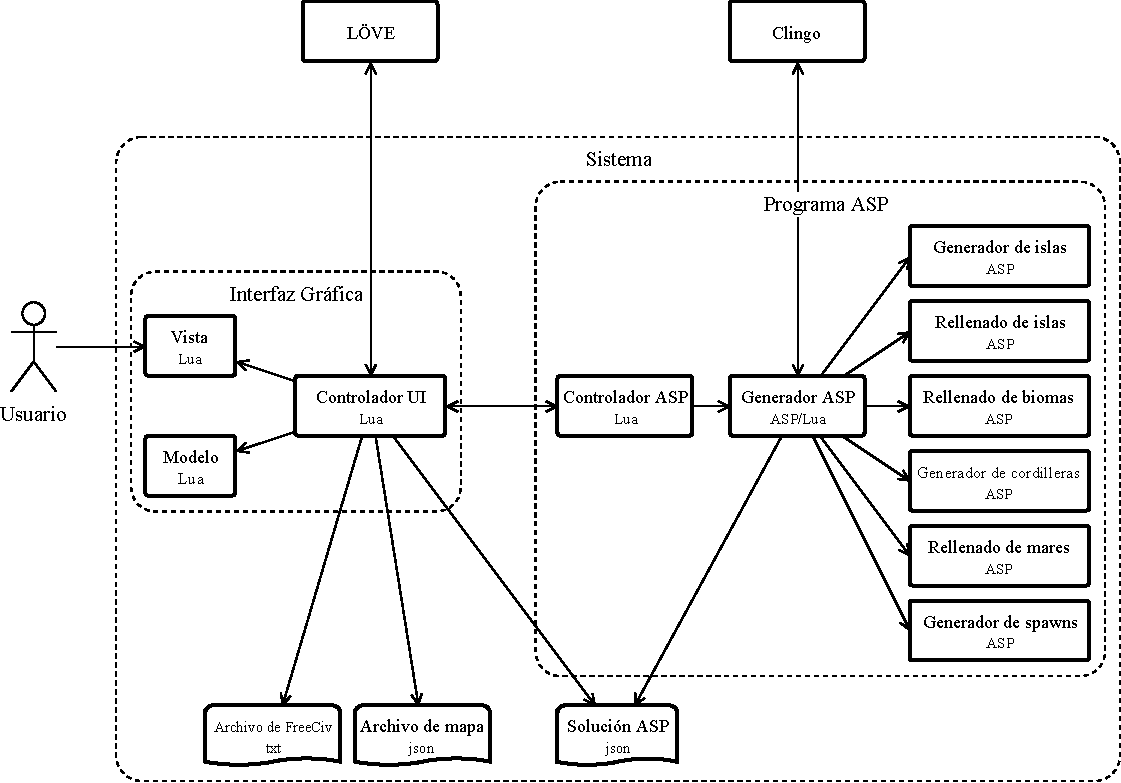
\includegraphics[width=\textwidth]{images/arquitectura.pdf}
	\caption{Arquitectura del sistema}
	\label{fig:arquitectura}
\end{figure}

Tanto el controlador de la interfaz de usuario como el controlador del programa ASP se ejecutarán en paralelo, pudiendo enviarse información de un controlador a otro para saber cuando hay que empezar una generación o si esta terminó. A pesar de esto, los resultados de la generación de ASP se guadarán en un archivo intermedio para evitar enviar gran cantidad de datos entre los elementos.

\subsection{Casos de uso}
\label{subsec:cases}

El sistema tiene en cuenta que se usará en todo momento por un único usuario, el cual llevará a cabo todas las funcionalidades propuestas en la Sección \ref{subsec:funcrequirements} a través de una interfaz gráfica que se explica en la Sección \ref{subsec:mockups}. Estos requisitos funcionales se transforman, por tanto, en los casos de uso del sistema que se proponen el la Figura \ref{fig:cases}.

\begin{figure}[!h]
	\centering
	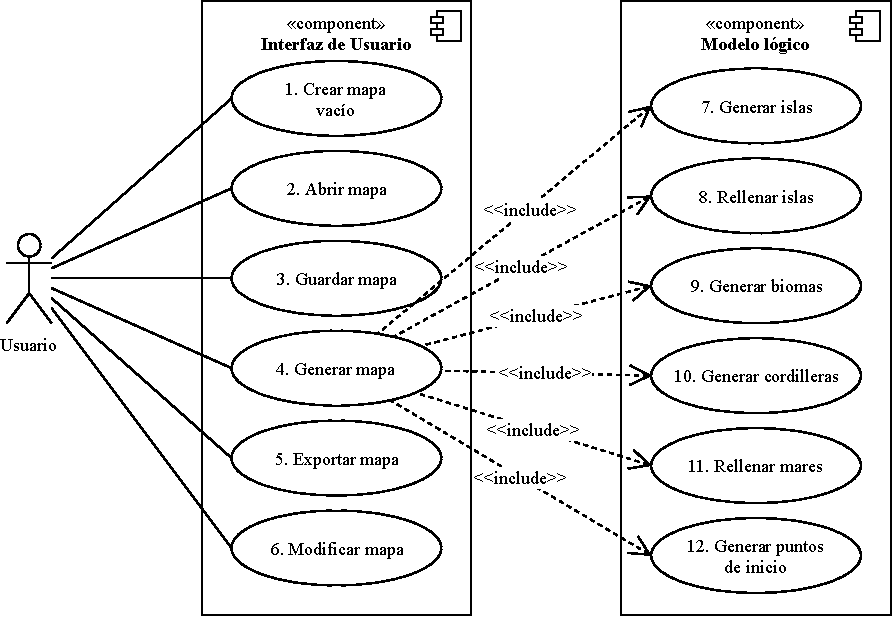
\includegraphics[width=\textwidth]{images/casos-de-uso.pdf}
	\caption{Casos de uso del sistema propuesto}
	\label{fig:cases}
\end{figure}

\subsection{Pantallas del sistema}
\label{subsec:mockups}

El proyecto propuesto está pensado para ser usado a través de una interfaz gráfica de usuario, la cual es modelada mediante un patrón MVC como se indica en la Sección \ref{subsec:arquitectura}. Esta interfaz está dividida en varias vistas, las cuales corresponden con los casos de uso propuestos contra los que el usuario interacciona directamente en la Sección \ref{subsec:cases}.

\begin{itemize}	
	\begin{figure}[!h]
		\centering
		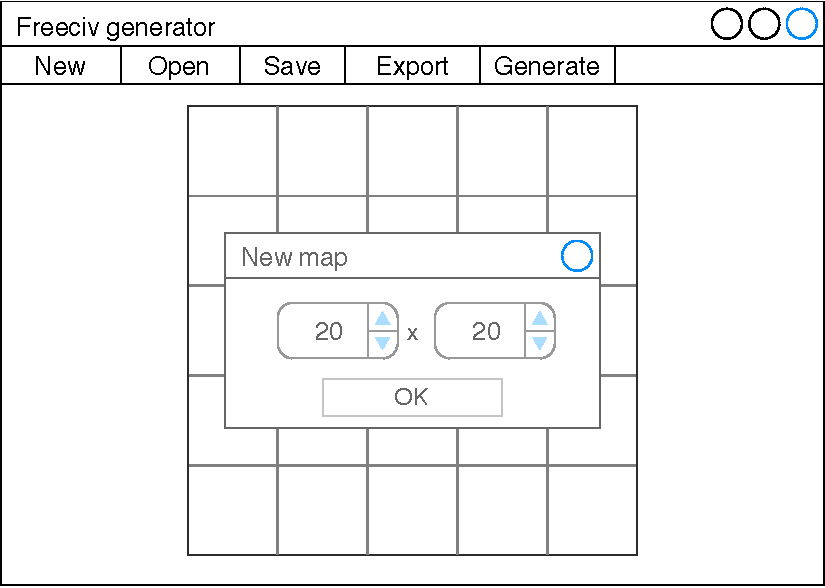
\includegraphics[width=0.5\textwidth]{images/new-map.pdf}
		\caption{Pantalla de nuevo mapa}
		\label{fig:newmock}
	\end{figure}
	
	\item 1. Crear mapa vacío: Se acciona cuando el usuario presiona en el botón de ``Crear mapa'' en la barra de herramientas, lo que despliega una ventana emergente parecida a la Figura \ref{fig:newmock}. Aquí el usuario puede indicar el tamaño del mapa a crear y pulsar el botón de ``Aceptar''. Con esto el sistema muestra una rejilla vacía.

	\begin{figure}[!h]
		\centering
		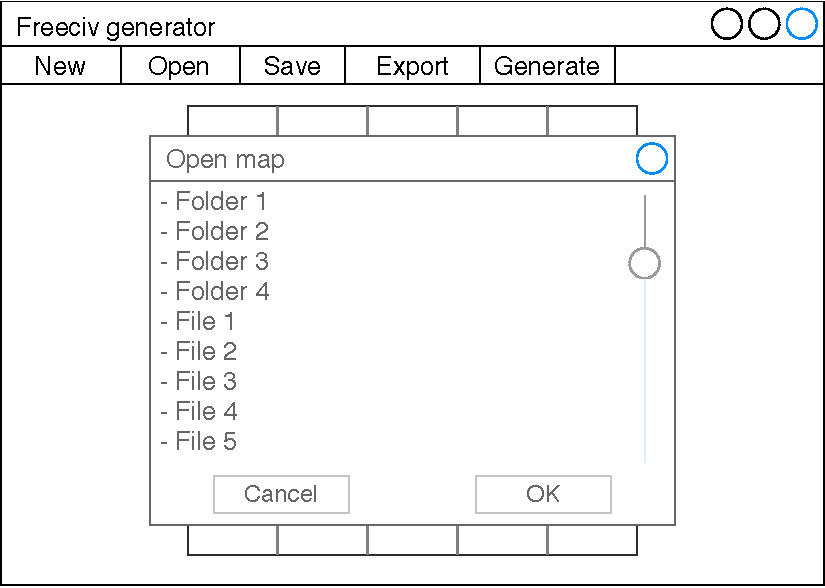
\includegraphics[width=0.5\textwidth]{images/open-map.pdf}
		\caption{Pantalla de abrir archivo de mapa}
		\label{fig:openmock}
	\end{figure}

	\item 2. Abrir mapa guardado en disco: Se inicia cuando el usuario presiona en el botón de ``Abrir mapa'' en la barra de herramientas, lo que despliega una ventana emergente parecida a la Figura \ref{fig:openmock}. Aquí el usuario navega a través de una lista que representa los archivos guardados en disco y selecciona un archivo anteriormente guardado por la aplicación que representa un mapa. El sistema procede a cargarlo y mostrar los datos del mapa en la rejilla principal.
	
	\begin{figure}[!h]
		\centering
		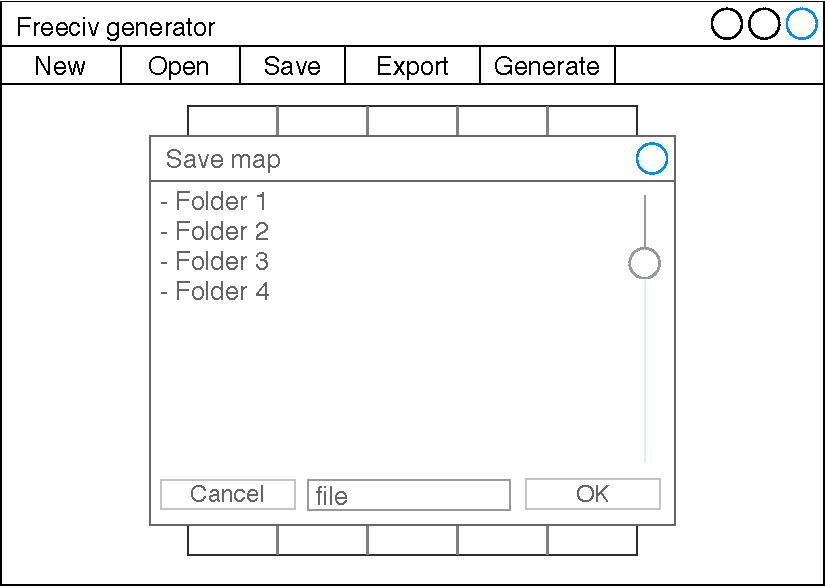
\includegraphics[width=0.5\textwidth]{images/save-map.pdf}
		\caption{Pantalla de guardar mapa}
		\label{fig:savemock}
	\end{figure}
	
	\item 3. Guardar mapa en disco: Se inicia cuando el usuario presiona en el botón de ``Guardar mapa'' en la barra de herramientas, mostrando una ventana emergente como la de la Figura \ref{fig:savemock}. Aquí el usuario navega por las carpetas guardadas en disco a través de una lista y selecciona una donde se guardará. Además, escribe el nombre del nuevo archivo en un campo de texto debajo de esta lista y acepta. El sistema procede a transformar los datos del mapa en un fichero que se guarda en disco donde el usuario indicó.
	
	\begin{figure}[!h]
		\centering
		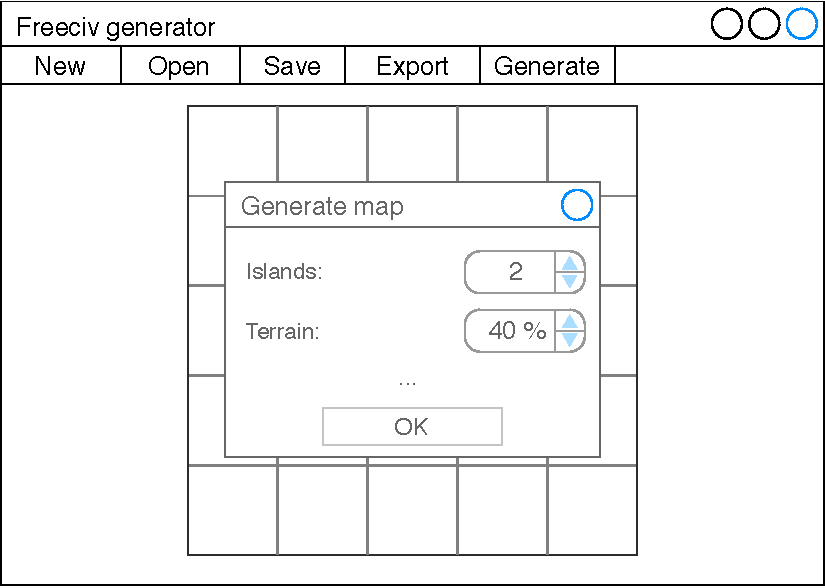
\includegraphics[width=0.5\textwidth]{images/generate-map.pdf}
		\caption{Pantalla de generar mapa}
		\label{fig:generatemock}
	\end{figure}
	
	\item 4. Generar mapa: Se inicia cuando el usuario acciona el botón de ``Generar mapa'' en la barra de herramientas, haciendo que el sistema muestre una ventana emergente parecida a la Figura \ref{fig:generatemock}. Aquí el usuario indica los parámetros que prefiera en la generación y acepta. En sistema procede a llamar a la parte del programa lógico creado en ASP, la cual va ejecutando cada uno de los casos de uso. Entre medias, el sistema lanza una vista como la de la Figura \ref{fig:waitingmock} para proporcionar retro-alimentación al usuario. Una vez acabada la generación, el sistema muestra en la rejilla principal con el mapa que se ha generado finalmente.

	\begin{figure}[!h]
		\centering
		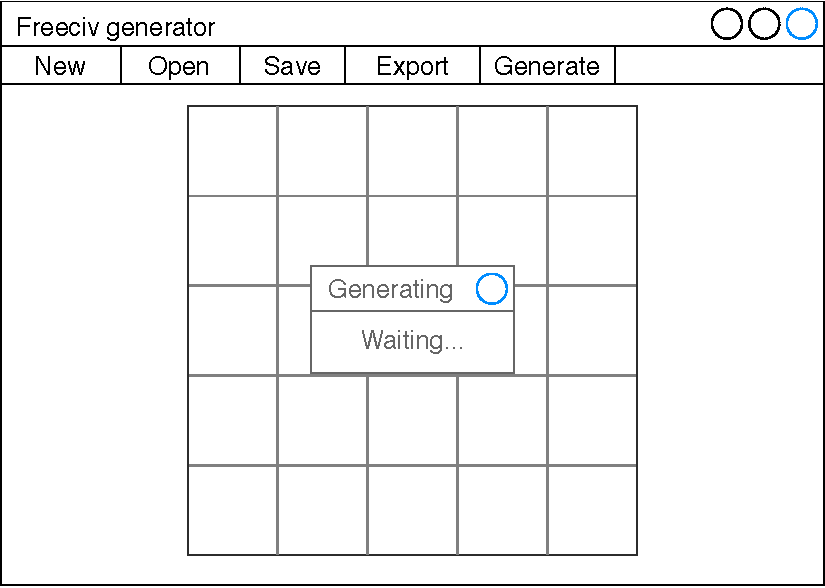
\includegraphics[width=0.5\textwidth]{images/waiting-mock.pdf}
		\caption{Pantalla con el mensaje de espera}
		\label{fig:waitingmock}
	\end{figure}
	
	\item 5. Exportar mapa al formato de Freeciv: Se inicia cuando el usuario presiona en el botón de ``Exportar mapa'' en la barra de herramientas, mostrando una ventana emergente como la de la Figura \ref{fig:exportmock}. Aquí el usuario navega por las carpetas guardadas en disco a través de una lista y selecciona una donde se guardará. Además, escribe el nombre del nuevo archivo en un campo de texto debajo de esta lista y acepta. El sistema procede a transformar los datos del mapa en un fichero reconocible por Freeciv y se guarda en disco donde el usuario indicó.
	
	\begin{figure}[!h]
		\centering
		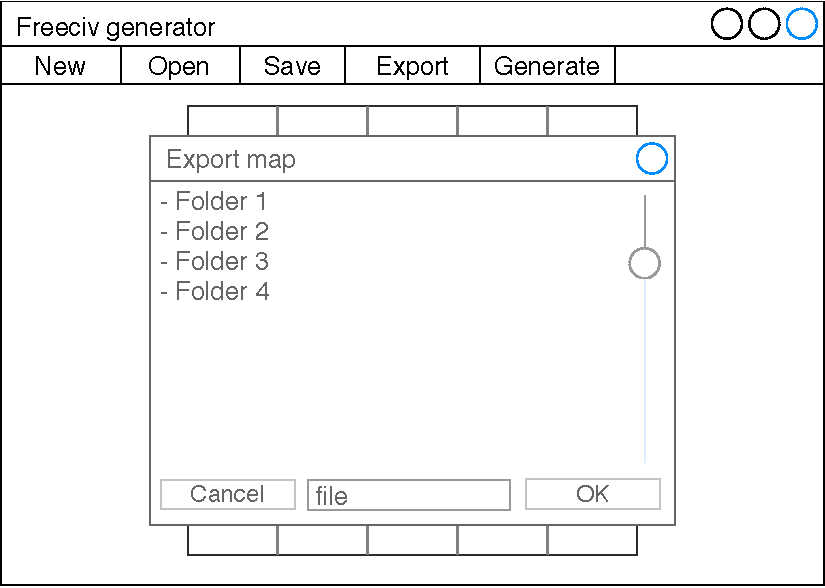
\includegraphics[width=0.5\textwidth]{images/export-map.pdf}
		\caption{Pantalla de exportar mapa}
		\label{fig:exportmock}
	\end{figure}
	
	\item 6. Modificar mapa: Se inicia cuando el usuario presiona sobre una de las celdas de la rejilla como en la Figura \ref{fig:mainmock}. El sistema pasará a cambiar el terreno de la celda por otro, realizando un ciclo en el momento en el que no quede ninguna opción nueva.
	
	\begin{figure}[!h]
		\centering
		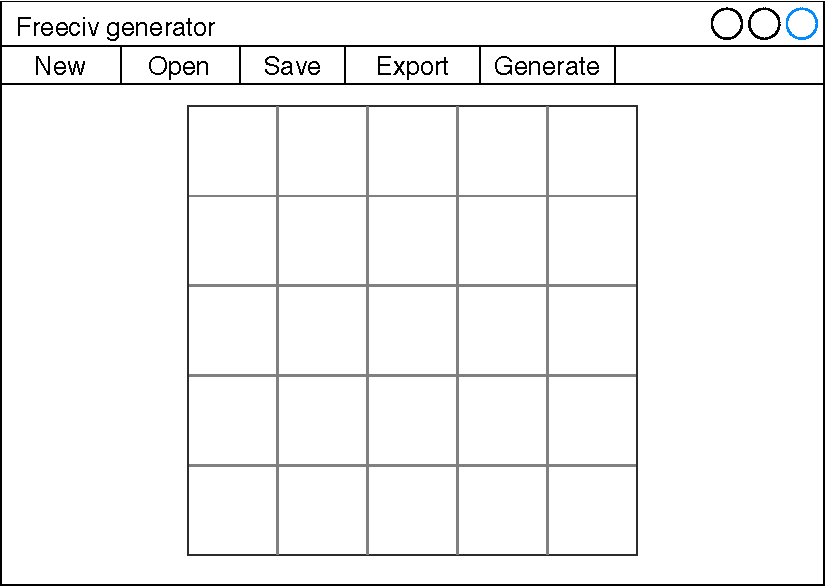
\includegraphics[width=0.5\textwidth]{images/aplicacion.pdf}
		\caption{Pantalla principal de la aplicación}
		\label{fig:mainmock}
	\end{figure}

\end{itemize}

\subsection{Implementación}
\label{subsec:implementacion}

Una vez analizado el proyecto en cuestión, pasaré a detallar el diseño de cada uno de los diferentes componentes del sistema en su construcción, indicando mediante diagramas como se integran los diferentes elementos. \\

Como ya se indicó en la Sección \ref{subsec:lua}, el lenguaje de programación Lua no tiene un paradigma de programación orientado a objetos basados en clases, más se ha preferido que en la realización de este sistema se use el módulo \textit{class.lua} de la biblioteca \textit{HUMP}\footnote{https://github.com/vrld/hump} para una organización lo más estructurada posible. Así mismo, también hay que destacar que el lenguaje tampoco soporta la manipulación de archivos en formato JSON, por lo que se ha usado el módulo \textit{json.lua}\footnote{https://github.com/rxi/json.lua}, el cual permite transformar un texto en formato JSON a tipos compatibles en Lua. \\

Por último, indicar que para la realización de las vistas de la interfaz de usuario se ha usado la biblioteca \textit{SUIT}\footnote{https://github.com/vrld/SUIT}, que permite generar una interfaz gráfica en modo inmediato de forma sencilla sobre LÖVE, pudiendo realizar un prototipo de los elementos más rápidamente y con más flexibilidad que con otro tipo de bibliotecas gráficas, como puede ser GTK+\footnote{https://www.gtk.org/}. Por otra parte, habrá elementos gráficos más complejos (como pueden ser diálogos de selección de ficheros o ventanas emergentes) que se tendrán que generar a mano, tal y como se expone en la Sección \ref{subsubsec:widgets}.

\subsubsection{Clase principal}
\label{subsubsec:main}

Como se puede ver en la Figura \ref{fig:mainclass} se ha diseñado la clase principal \texttt{Main}, la cual es una clase estática que sirve de controlador para las vistas y el modelo. Implementa los casos de uso de la interfaz descritos en la Sección \ref{subsec:cases} en los métodos \texttt{\_newMap}, \texttt{\_openMap}, \texttt{\_saveMap}, \texttt{\_exportMap} y \texttt{\_generateMap}, que son eventos que se llaman desde los diálogos emergentes tal y como se explica desde la Sección \ref{subsubsec:widgets}. Para el caso de uso de modificar el mapa, la tarea recae en la clase \texttt{Editor}, que se explica en detalle en la Sección \ref{subsubsec:client}. \\

\begin{figure}[!h]
	\centering
	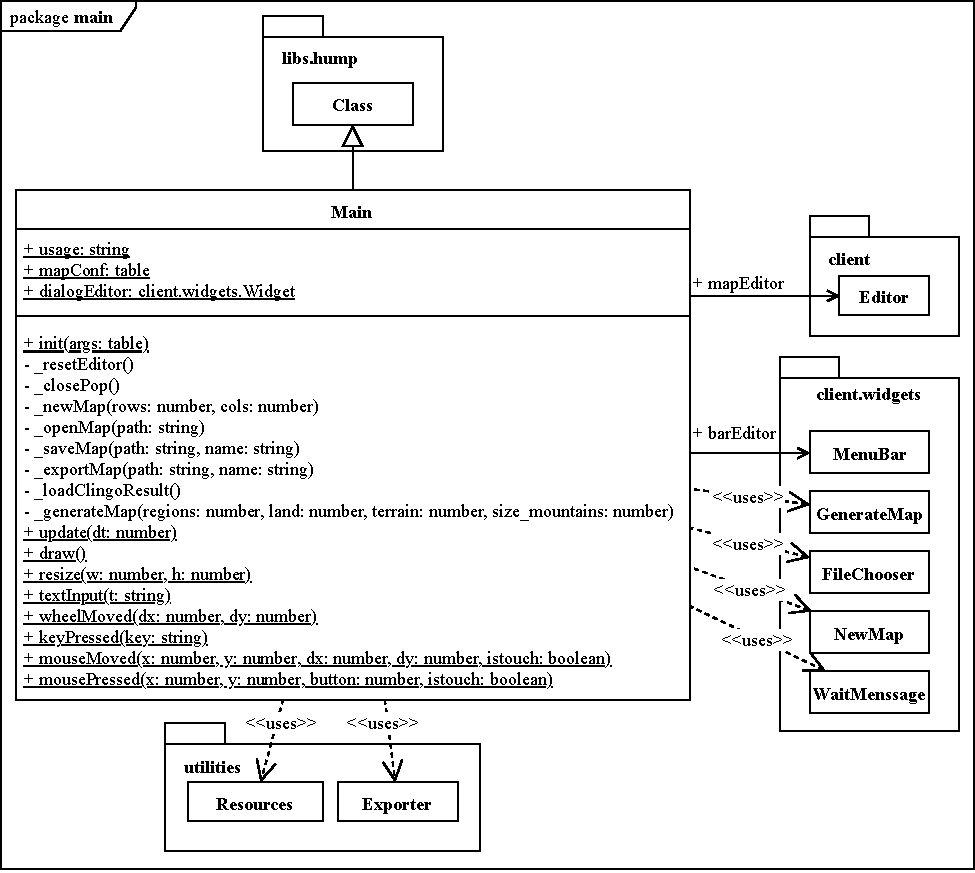
\includegraphics[width=\textwidth]{images/clase-principal.pdf}
	\caption{Diagrama de clases del paquete principal}
	\label{fig:mainclass}
\end{figure}

Con respecto al motor gráfico LÖVE, este usa varias funciones predefinidas cuando se activan distintos eventos, los cuales llaman a los métodos públicos de la clase principal:

\begin{itemize}
	\item El método \texttt{init} es llamado en la función \texttt{love.load} la primera vez que se ejecuta el programa. Sirve para cargar los elementos gráficos e iniciar el resto de clases que serán usadas por el programa.
	\item Como LÖVE es un motor para programación de videojuegos, la función \texttt{love.update} es llamada en un bucle de eventos internos antes de actualizar la pantalla. Esta función llama al método homónimo de la clase principal, el cual prepara las vistas de la interfaz para su pintado en pantalla y llama a los métodos correspondientes según los eventos producidos en las vistas.
	\item Una vez actualizada la lógica, se procede al pintado de pantalla mediante la función \texttt{love.draw}, la cual llama al método con el mismo nombre de la clase principal, que se encarga de pintar las vistas en pantalla.
	\item Existen otros eventos, los cuales LÖVE tiene contempladas varias funciones por defecto adicionales que se lanzan para contestar a estos. Es el caso de cuando se redimensiona la ventana (\texttt{love.resize}), se introduce un texto mediante un teclado virtual (\texttt{love.textinput}), se realiza un movimiento de la rueda del ratón (\texttt{love.wheelmoved}), se presiona una tecla (\texttt{love.keypressed}), se mueve el ratón (\texttt{love.mousemoved}) o se presiona un botón del ratón (\texttt{love.mousepressed}). Estas llaman a los métodos correspondientes de la clase principal.
\end{itemize}

\subsubsection{Editor gráfico}
\label{subsubsec:client}

La clase \texttt{Editor} sirve como un controlador para responder a las modificaciones y cambios de representación del mapa, ya sea cuando se actualiza este mediante uno de los casos de uso que recoge la clase principal [ver Sección \ref{subsubsec:main}] o cuando el usuario procede a la modificación del mapa, tal y como se explica en la Sección \ref{subsec:cases}.

\begin{figure}[!h]
	\centering
	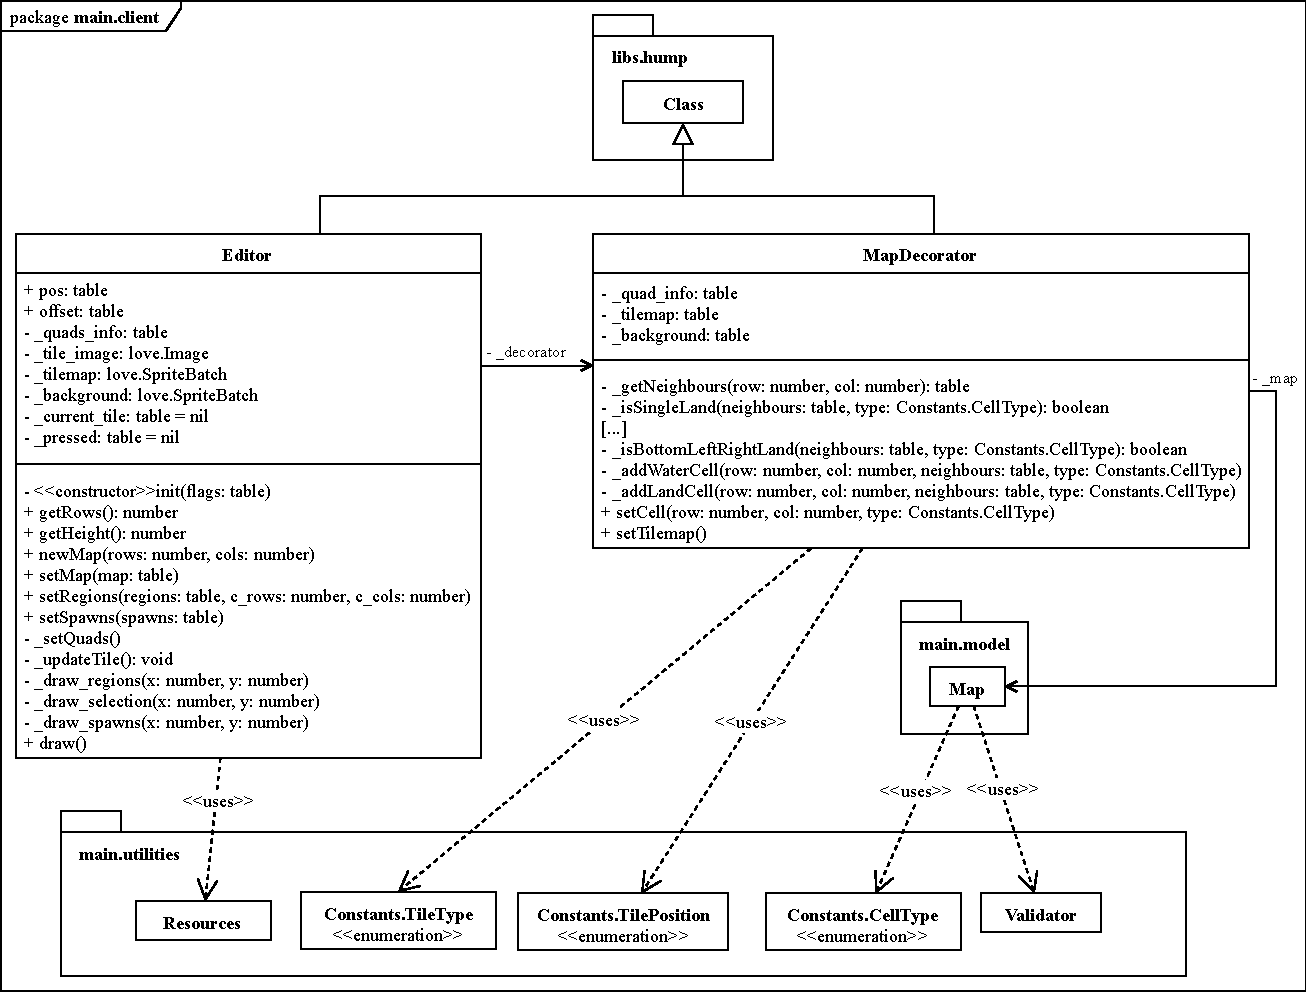
\includegraphics[width=\textwidth]{images/clase-editor.pdf}
	\caption{Diagrama de clases del paquete \texttt{Client}}
	\label{fig:editorclass}
\end{figure}

Para ello, siguiendo el patrón decorador, esta se apoya en la clase \texttt{MapDecorator}, la cual se encarga de actualizar la vista del mapa, que es representada mediante una rejilla con los distintos terrenos mediante el objeto \texttt{love.SpriteBatch}, el cual es un mapa de \textit{tiles} bidimensional. Debido a que hay terrenos que contienen diferentes imágenes para las posiciones de un \textit{tile}, \texttt{MapDecorator} contiene varios métodos que permiten discretizarlas conociendo los vecinos de una celda. Finalmente esta clase llama al modelo en si, representado por la clase \texttt{Map}, la cual tiene una representación del mapa en forma de tabla. \\

Finalmente todas estas clases usan constantes que están definidas el módulo \texttt{Constants}.

\subsubsection{Elemento gráficos complejos}
\label{subsubsec:widgets}

Como ya expliqué en la entrada de la Sección \ref{subsec:implementacion}, debido a las limitaciones de la biblioteca \textit{SUIT}, hay varios elementos gráficos que no se incluyen en ella debido a que son complejos y no es del ámbito de esta bibloteca, es por eso que se han realizado a mano. Estos elementos tienen su propio controlador para poder usarlos más fácilmente dentro del programa.

\begin{figure}[!h]
	\centering
	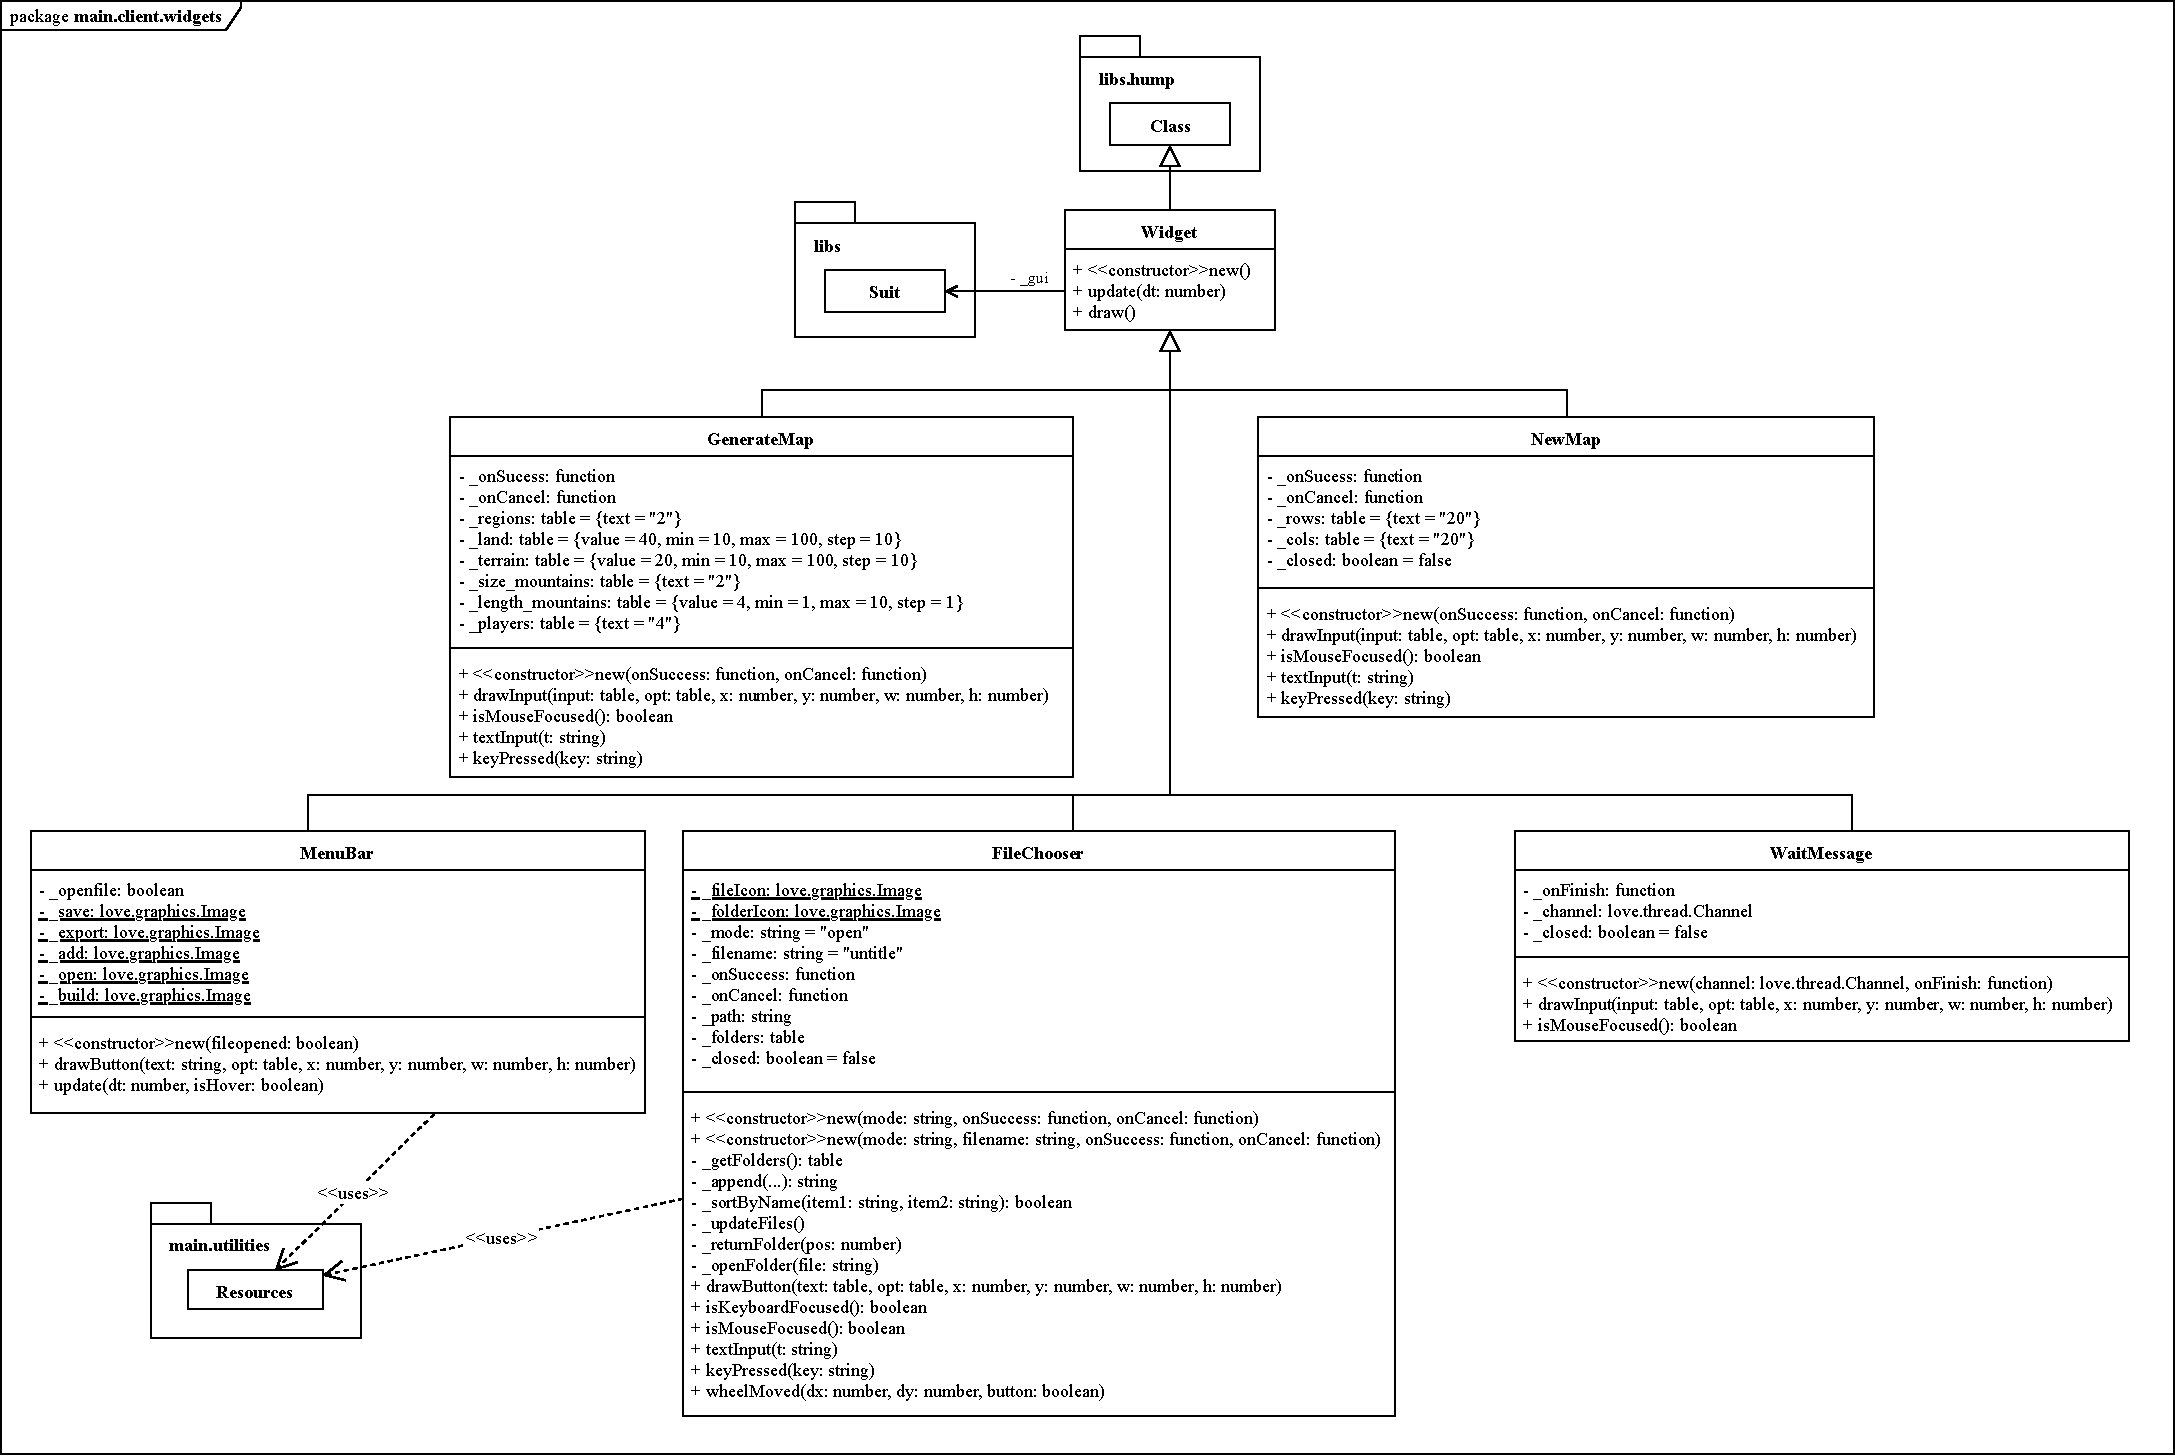
\includegraphics[width=\textwidth]{images/clases-widgets.pdf}
	\caption{Diagrama de clases del paquete \texttt{Widget}}
	\label{fig:widgetclasses}
\end{figure}

\begin{itemize}
	\item Para la barra de herramientas se ha realizado la clase \texttt{MenuBar}, la cual controla y muestra la lista de botones que accionan los principales casos de uso. Al constructor se le pasa las funciones para los eventos de aceptar y cancelar diálogo. Tiene un método \texttt{update} que devuelve un número que se corresponde con el botón pulsado en la barra.
	\item La clase \texttt{NewMap} controla y muestra la ventana emergente que se puede ver en la Figura \ref{fig:newmock}. Al constructor se le pasa las funciones para los eventos de aceptar y cancelar diálogo. Contiene el método \texttt{isMouseFocused} que indica si el ratón está encima de la ventana, y los métodos \texttt{textInput} y \texttt{keyPressed} para introducir texto en las entradas de la ventana.
	\item La clase \texttt{GenerateMap} controla y muestra la ventana emergente con el diálogo de generar mapa, tal y como se puede ver en la Figura \ref{fig:generatemock}. Contiene los mismos métodos que la clase \texttt{NewMap}.
	\item La clase \texttt{WaitMessage} controla y muestra la ventana emergente que se puede ver en la Figura \ref{fig:waitingmock}. Al constructor se le pasa el canal del \textit{thread} que se usa en la generación del mapa, tal y como se expone en la Sección \ref{subsubsec:generator}, y la función que se lanza cuando la generación termina. Contiene el método \texttt{isMouseFocused} que indica si el ratón está encima de la ventana.
	\item La clase \texttt{FileChooser} controla y muestra la ventana emergente correspondiente a un diálogo de selección de archivo, tal y como se puede ver en las Figuras \ref{fig:openmock}, \ref{fig:savemock} y \ref{fig:exportmock}. Contiene varios métodos privados para la ordenación y la apertura de carpetas en disco, así como el método \texttt{isMouseFocused} que indica si el ratón está encima de la ventana, los métodos \texttt{textInput} y \texttt{keyPressed} para introducir texto en las entradas de la ventana y el método \texttt{wheelMoved} que permite subir y bajar la lista de carpetas y ficheros mediante la rueda del ratón.
\end{itemize}

\subsubsection{Generador de mapas}
\label{subsubsec:generator}

\begin{figure}[!h]
	\centering
	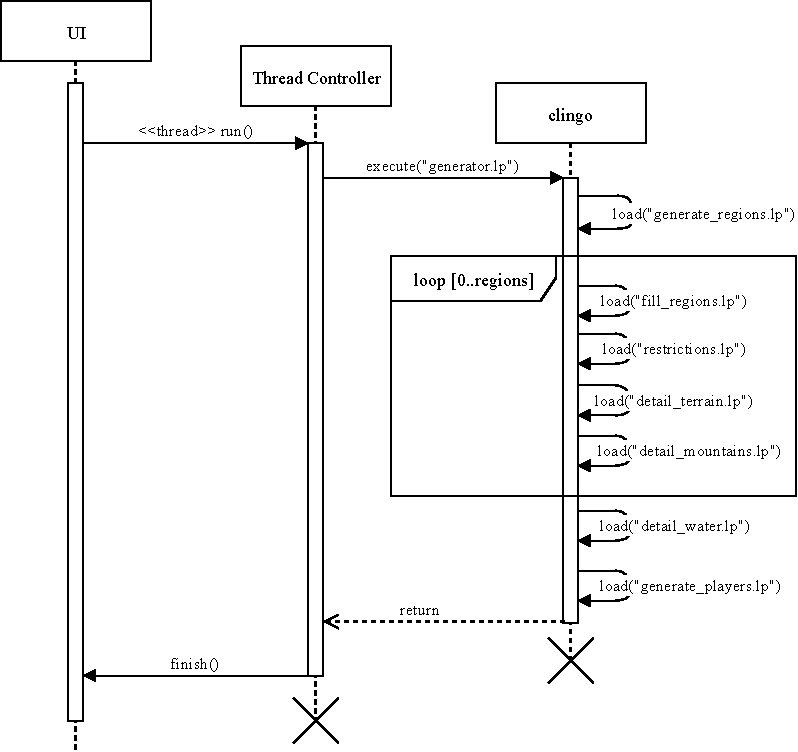
\includegraphics[width=\textwidth]{images/secuencia.pdf}
	\caption{Diagrama de secuencia de la ejecución del generador}
	\label{fig:sequence}
\end{figure}
	\cleardoublepage
	
	\chapter{Evaluación}
	\label{evaluation}
	En este capítulo se analizará los resultados obtenidos en el proceso de evaluación del sistema. Para la planificación de las pruebas se ha optado por el uso de una herramienta de integración continua en donde se corren tanto pruebas de unidad a las partes del modelo de la interfaz gráfica, así como a los distintos módulos de los programas lógicos. \\

Además se ha usado un programa escrito en Lua para la ejecución de pruebas de rendimiento o \textit{benchmarks} el cual solo usa el módulo clingo para evitar el uso de la interfaz gráfica. En todas estas pruebas se ha añadido a las pruebas la restricción de que el cómputo del mapa solo puede durar como máximo cinco minutos, matando el proceso en caso de superar este tiempo y pasando a la siguiente prueba. Con esto podemos indicar cuales son las configuraciones que dan una experiencia pobre al usuario. \\

A continuación se describen los resultados obtenidos de estas pruebas de rendimiento con distintos parámetros. \\

\section{Tamaño de los mapas}

Estas pruebas se han realizado usando distintos tamaños de mapas cuadrados, dejando el resto de variables con valores por defecto (cantidad de tierra y de biomas al 20\%, tamaño de las cordilleras en 2 casillas, longitud de cordilleras en 3 casillas, 2 jugadores y 2 casillas de distancia mínima entre jugadores). \\

Debido a que el módulo pide el número de cuadrantes y el tamaño en casillas de un cuadrante, se han realizado las pruebas calculando primero el tamaño total del mapa y con esto se ha obtenido tres números números:

\begin{align}
	islands &= \lfloor \sqrt{size} - 1 \rfloor \\
	n_1 | size, & \text{ en donde } n_1 > islands. \\
	n_2 &= size / n_1
\end{align}

Con esto se procede a obtener el número de cuadrantes y el tamaño del cuadrante mediante:

\begin{align}
	q_{num} &= min(n_1, n_2) \\
	q_{size} &= max(n_1, n_2) \\
\end{align}

\begin{table}[!h]
	\begin{tabularx}{\textwidth}{ X X X X X X }
		\bfseries{Tamaño} & \bfseries{Islas} & $\mathbf{q_{num}}$ & $\mathbf{q_{size}}$ & \bfseries{Total} & \bfseries{Ejecución} \\
		\hline
		10 x 10 & 2 & 2 & 5 & 6 s & 117 ms \\
		15 x 15 & 2 & 3 & 5 & 17 s & 145 ms \\
		20 x 20 & 3 & 4 & 5 & 88 s & 296 ms \\
		25 x 25 & 4 & 5 & 5 & 200 s & 675 ms \\
		30 x 30 & 4 & 5 & 6 & 1137 s & 731 ms \\
		35 x 35* & 4 & 5 & 7 & - & - \\
		40 x 40 & 5 & 5 & 8 & 1791 s & 1050 ms \\
		45 x 45 & 5 & 5 & 9 & 4627 s & 1047 ms \\
		\hline
	\end{tabularx}
	\begin{tablenotes}
		\item[1] Las filas indicadas con - se refieren a las pruebas en donde una ejecución no se han podido completan en menos de 5 minutos.
	\end{tablenotes}
	\caption{Resultado del \textit{benchmark} con diferentes tamaños de mapa.}\label{table:mapresult}
\end{table}

\begin{figure}[!h]
	\centering
	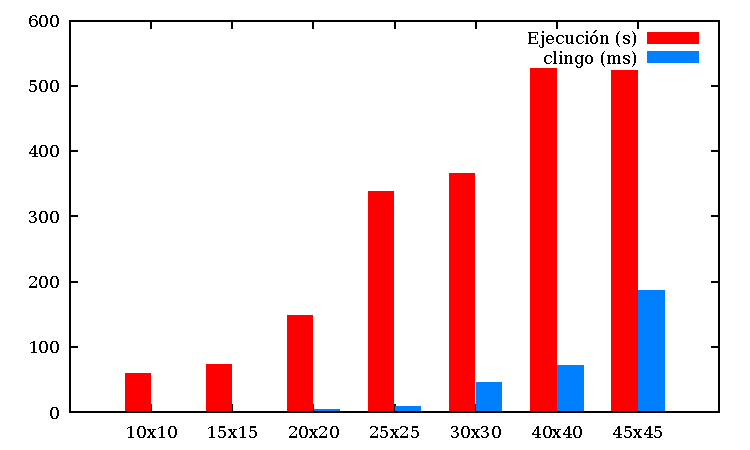
\includegraphics[width=.8\textwidth]{tables/map-size.pdf}
	\caption{Tiempos del \textit{benchmark} con diferentes tamaños de mapa.}\label{fig:mapresult}
\end{figure}

Con esto nos aseguramos de que cada uno de los módulos tengan porciones parecidas para computar. En la Tabla \ref{table:mapresult} podemos ver los resultados de la realización de esta prueba de rendimiento ejecutando 25 ejecuciones cada una de las medidas, en donde se recoge el tiempo total de todas las ejecuciones, el tiempo total que ha usado clingo para obtener una solución y el tiempo medio de una ejecución. Por otra parte en la Figura \ref{fig:mapresult} podemos ver una comparativa entre el tiempo medio entre ejecuciones y el tiempo medido arrojado por clingo. \\

Como se puede observar, el tiempo de ejecución sigue una tendencia casi exponencial, haciendo que a partir de mapas de 45x45 celdas en ningún momento la ejecución tarde menos de 5 minutos. Aún así, hay que destacar un caso concreto, ya que la prueba de un mapa de 35x35 celdas con los valores propuestos se realiza en más de 5 minutos, cosa que tanto en las pruebas anteriores como en las siguientes no ocurre. Esto puede deberse a que el mapa para esta prueba no esté bien repartido para los distintos módulos.  

\section{Porcentajes de tierra y biomas}
\label{sec:pruebatierrabiomas}

Para la primera parte de la prueba se ha usado distintos porcentajes de tierra, usando la cantidad de islas y los parámetros de cantidad y tamaño de los cuadrantes para mapas de 25x25 celdas de la prueba anterior y dejando el resto de variables con valores por defecto (cantidad de biomas al 20\%, tamaño de las cordilleras en 2 casillas, longitud de cordilleras en 3 casillas, 2 jugadores y 2 casillas de distancia mínima entre jugadores). \\

\begin{table}[!h]
	\centering
	\begin{tabular}{ c c c }
		\bfseries{Porcentaje} & \bfseries{Total} & \bfseries{Ejecución} \\
		\hline
		10\% & 174 s & 6,96 s \\
		15\% & 178 s & 7,12 s \\
		20\% & 178 s & 7,12 s \\
		25\% & 179 s & 7,16 s \\
		30\% & 181 s & 7,24 s \\
		35\% & 178 s & 7,12 s \\
		40\% & 179 s & 7,16 s \\
		45\% & 178 s & 7,12 s \\
		50\% & 181 s & 7,24 s \\
		55\% & 179 s & 7,16 s \\
		60\% & 178 s & 7,12 s \\
		65\% & 179 s & 7,16 s \\
		70\% & 178 s & 7,12 s \\
		75\% & 180 s & 7,20 s \\
		80\% & 180 s & 7,20 s \\
		\hline
	\end{tabular}
	\caption{Resultado del \textit{benchmark} con diferentes porcentajes de tierra.}\label{table:landresult}
\end{table}

\begin{figure}[!h]
	\centering
	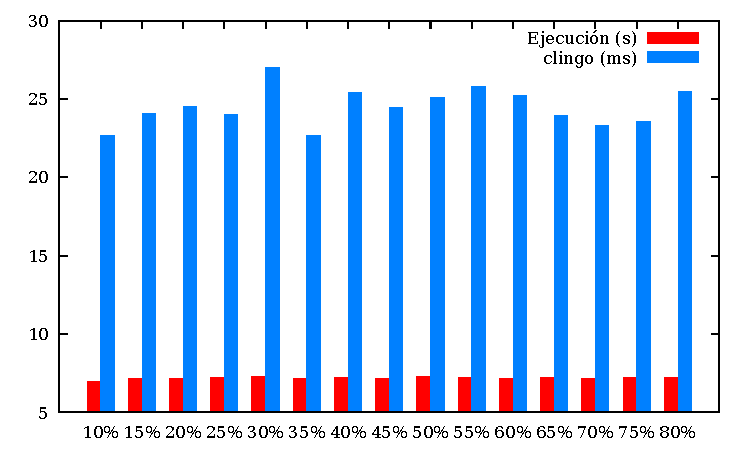
\includegraphics[width=.8\textwidth]{tables/land-size.pdf}
	\caption{Tiempos del \textit{benchmark} con diferentes porcentajes de tierra.}\label{fig:landresult}
\end{figure}

En la Tabla \ref{table:landresult} podemos ver los resultados de la realización de esta prueba de rendimiento ejecutando 25 ejecuciones cada una de las medidas, en donde se recoge el tiempo total de todas las ejecuciones, el tiempo total que ha usado clingo para obtener una solución y el tiempo medio de una ejecución. Por otra parte en la Figura \ref{fig:landresult} podemos ver una comparativa entre el tiempo medio entre ejecuciones y el tiempo medido arrojado por clingo. \\

En el caso de la segunda parte de la prueba se ha usado distintos porcentajes de cantidad de bioma que alcanza una isla, usando los mismos datos que para la prueba anterior. En la Tabla \ref{table:biomaresult} podemos ver los resultados de la realización de esta prueba de rendimiento ejecutando 25 ejecuciones cada una de las medidas, en donde se recoge el tiempo total de todas las ejecuciones, el tiempo total que ha usado clingo para obtener una solución y el tiempo medio de una ejecución. Por otra parte en la Figura \ref{fig:biomaresult} podemos ver una comparativa entre el tiempo medio entre ejecuciones y el tiempo medido arrojado por clingo. \\

\begin{table}[!h]
	\centering
	\begin{tabular}{ c c c }
		\bfseries{Porcentaje} & \bfseries{Total} & \bfseries{Ejecución} \\
		\hline
		10\% & 178 s & 7,12 s \\
		15\% & 180 s & 7,20 s \\
		20\% & 179 s & 7,16 s \\
		25\% & 178 s & 7,12 s \\
		30\% & 178 s & 7,12 s \\
		35\% & 179 s & 7,16 s \\
		40\% & 179 s & 7,16 s \\
		45\% & 213 s & 8,52 s \\
		50\% & 215 s & 8,60 s \\
		55\% & 216 s & 8.64 s \\
		60\% & 207 s & 8,28 s \\
		65\% & 192 s & 7,68 s \\
		70\% & 187 s & 7,48 s \\
		75\% & 208 s & 8,32 s \\
		80\% & 204 s & 8,16 s \\
		\hline
	\end{tabular}
	\caption{Resultado del \textit{benchmark} con diferentes porcentajes de tierra.}\label{table:biomaresult}
\end{table}

\begin{figure}[!h]
	\centering
	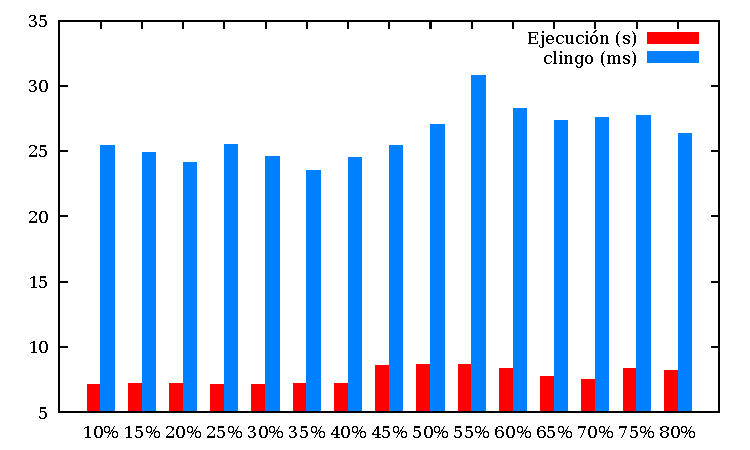
\includegraphics[width=0.8\textwidth]{tables/bioma-size.pdf}
	\caption{Tiempos del \textit{benchmark} con diferentes porcentajes de tierra.}\label{fig:biomaresult}
\end{figure}

Como se puede observar, en estas pruebas no se haya bastante diferencia al modificar uno de los valores, dando resultados muy similares entre si. Es por eso que se ha decidido combinar las dos pruebas en una sola para observar algún cambio efectivo. Esto se recoge en la Sección \ref{sec:pruebafinal}.

\section{Prueba mixta tierra/biomas}
\label{sec:pruebafinal}

En esta última prueba se ha tenido en cuenta los datos de la prueba relatada en la Sección \ref{sec:pruebatierrabiomas}, es decir, usando un mapa de 25x25 dividido en 5 cuadrantes de 5 celdas cada uno, con 4 islas totales y dejando el resto de variables con valores por defecto (tamaño de las cordilleras en 2 casillas, longitud de cordilleras en 3 casillas, 2 jugadores y 2 casillas de distancia mínima entre jugadores).

\begin{table}[!h]
	\centering
	\begin{tabular}{c|cccccc}
	 & 10\% & 15\% & 20\% & 25\% & 30\% & 35\% \\
	\hline
	10\% & 42 & 41 & 35 & 88 & 117 & 214 \\
	15\% & 41 & 37 & 36 & 88 & 133 & 247 \\
	20\% & 37 & 43 & 37 & 105 & 123 & 224 \\
	25\% & 29 & 51 & 43 & 92 & 123 & 220 \\
	30\% & 42 & 43 & 138 & 95 & - & - \\
	35\% & 41 & 40 & 38 & 90 & - & 241 \\
	40\% & 43 & 46 & 36 & -  & - & 217  \\
	45\% & 69 & 49 & 36 & 737 & - & 220 \\
	50\% & 100 & - & 1064 & - & - & - \\
	55\% & 55 & 956 & - & - & - & - \\
	60\% & 164 & 740 & - & - & - & - \\
	65\% & 97 & 838 & - & - & - & - \\
	\hline
	\end{tabular}
	\caption{Resultado del \textit{benchmark} con diferentes porcentajes de tierra (las columnas) y de biomas (las filas). Los tiempos totales son en segundos.}\label{table:finalresult}
\end{table}

Como se puede observar en los resultado mostrados en la Tabla \ref{table:finalresult}, en donde se han ejecutado 5 iteraciones por cada valor, el módulo de clingo obtiene resultados decentes cuando se establecen valores bajos para el porcentaje de tierra y de biomas, más el tiempo de ejecución se dispara en el momento de poner valores altos. Esto se debe a, como ya se ha comentado a lo largo de la memoria, el paradigma ASP puede llegar a tener en cuenta una gran combinación de datos y producirse una explosión combinatoria de soluciones, retardando en buena medida la procura de una solución.
	\cleardoublepage
	
	\chapter{Conclusiones}
	\label{conclusions}
	En este proyecto se construido una herramienta declarativa con la que elaborar, mediante programación lógica, nuevos escenarios para el videojuego Freeciv. Para ello se usó el paradigma de \textit{Answer Set Programming}, una variante de Programación Lógica de uso frecuente para la Representación del Conocimiento y la resolución de problemas. La principal ventaja de \textit{Answer Set Programming} para este caso fue la facilidad que otorgaba el uso de predicados simples a la hora de definir ciertas propiedades dentro de un escenario concreto, así como añadir directamente reglas de restricción para ciertos elementos del mapa bajo la forma de reglas de programación lógica. Esto proporcionó una gran flexibilidad, ya que con ello sólo se necesita realizar la especificación del problema sin importar el método de resolución que se aplicará. \\

También se ha reducido el problema que surge al tener en cuenta todas las reglas y restricciones del mapa, lo cual produce una explosión combinatoria de soluciones, y ocasionaba que el sistema tardase en encontrar. Para ello se ha separado el problemas de búsqueda del modelo declarativo en distintos módulos independientes: un generador de regiones, un módulo para rellenar las regiones, un generador de biomas, un módulo que define cordilleras, un módulo para definir las celdas de agua y por último un módulo para definir los puntos iniciales de los jugadores. \\

A pesar de todo esto, existen algunas limitaciones de cara la finalización de este proyecto, las cuales pueden ser resueltas en un futuro inmediato:

\begin{itemize}
	\item El sistema no tiene en cuenta todos los elementos que proporciona el videojuego, por lo que no soporta actualmente la generación de ríos, ni la generación de recursos ni la generación de puntos de inicio para bárbaros o aldeas perdidas. Esto se podría solucionar añadiendo nuevos módulos a la generación del mismo.
	\item El sistema presenta graves problemas de eficiencia a la hora de generar grandes porciones de mapas, mermando la funcionalidad de la herramienta. Esto se puede observar en la Sección \ref{evaluation}, en donde había problemas con mapas mayores de 45x45 celdas en cuanto a tiempo de ejecución. Esto se podría resolver intentando pulir las reglas actuales de los módulos o replanteando la forma en la que se han definido, en algunos casos dividiendo más para reducir la carga de estos.
\end{itemize}

Para finalizar, se puede marcar una serie de líneas, tanto para solucionar y mejorar el sistema propuesto como para ampliar y extender las funcionalidades actuales de cara a largo plazo:

\begin{itemize}
	\item Mejorar la interfaz gráfica, incluyendo distintos elementos gráficos con los que manejar de forma más efectiva el mapa, como puede ser herramientas para ampliar y disminuir el mapa, mover el mapa o marcar de forma más visual el tipo de terreno marcar.
	\item Indicar de forma más visual restricciones en el mapa, así como zonas que tendrá en cuenta el generador para completar. Estas zonas incluso pueden tener restricciones de que piezas no poner o preferencias de los tipos de terrenos a generar.
	\item Publicar y anunciar la herramienta para tener una buena base de usuarios que puedan producir un \textit{feedback} del uso y características de la misma.
	\item Añadir a la base de conocimiento estilos personalizados, ya sea incluyéndolos dentro de las reglas o importándolos como perfiles. Estos permitirían que un usuario pueda tener preferencias de cara a la generación (que no le guste generar cordilleras cerca del agua, que los usuarios estén lo más cercano a bosques o recursos, etc).
\end{itemize}
	\cleardoublepage
	
	\listoftables
	\cleardoublepage
	
	\listoffigures
	\cleardoublepage
	
	\clearpage
	
	% ------- Appendices -------
	\appendix
	\addcontentsline{toc}{chapter}{Apéndices}
	\label{appendices}
	
	%\chapter{Diagramas}
	%\label{diagrams}
	%\input{tex/diagrams}
	%\cleardoublepage
	
	%\chapter{Manual de uso}
	%\label{manual}
	%\input{tex/manual}
	%\cleardoublepage
	
	%\chapter{Información de Lua}
	%\label{lua}
	%\input{tex/lua}
	%\cleardoublepage
	
	\clearpage
	
	% ------- Biliography -------
	\bibliographystyle{IEEEtran-spanish}
	\bibliography{bib/references}
	\addcontentsline{toc}{chapter}{A. Bibliografía}
	\label{bibliography}
\end{document}